\documentclass[a4paper,norsk]{article}
\usepackage[utf8]{inputenc}
\usepackage[T1]{fontenc,url}
\usepackage{babel,textcomp}
\usepackage{graphicx, wrapfig}
\usepackage{graphics}
\graphicspath{
	{Code/figs/}
}
\usepackage{amsmath}
\usepackage{stackengine}
\usepackage{listings}
\usepackage{amsfonts}
\urlstyle {sf}
\title {2. Mandatory assignment MAT2410 Autumn 2017}
\author {Mikael Ravndal}
\begin{document}
\maketitle
All approximation is done with degree equals 5.
\section*{Part a)}
Ordinary Least square of the Frankefunction(the same as Ridge with $\lambda=0$):
\\ 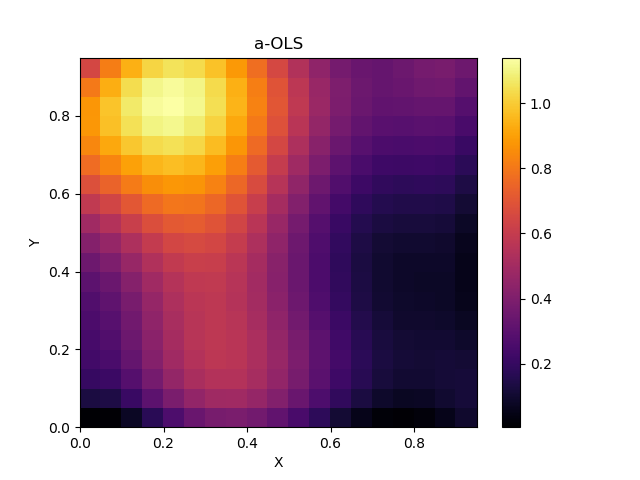
\includegraphics[scale=.7]{a-OLS}
\clearpage
\section*{Part b)}
Ridge Regression with $\lambda = 0.1$
\\ 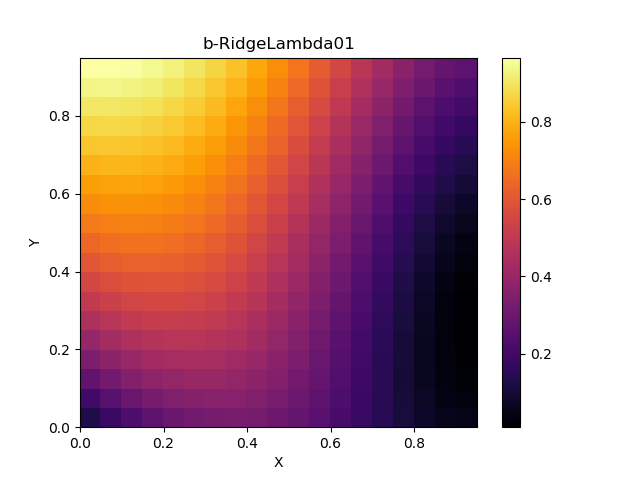
\includegraphics[scale=.7]{b-RidgeLambda01}
\clearpage

\section*{Part c)}
Lasso Regression with $\lambda = 0.01$
\\ 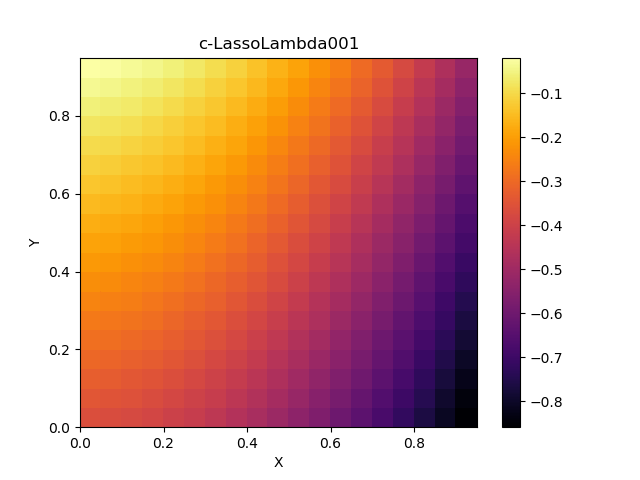
\includegraphics[scale=.7]{c-LassoLambda001}
\clearpage

\section*{Part d)}
Imports 100x100 chunk of real data from top left corner of dataset nr.1.
\\Plot of real data
\\ 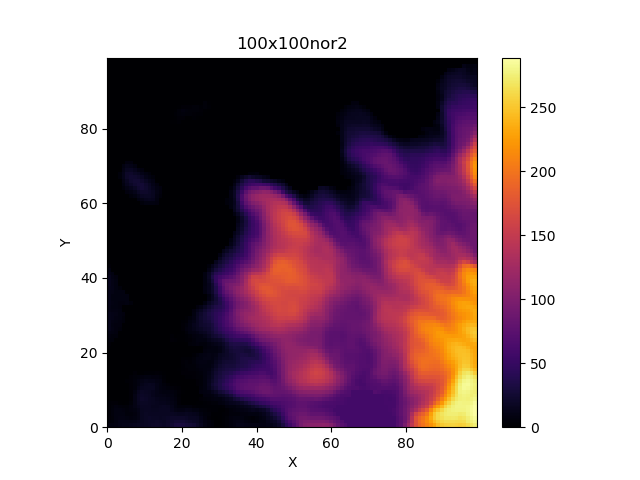
\includegraphics[scale=.7]{100x100nor2}
\clearpage
\section*{Part e)}
Repeat of a-c, but with real data from d)
\\OLS:
\\ 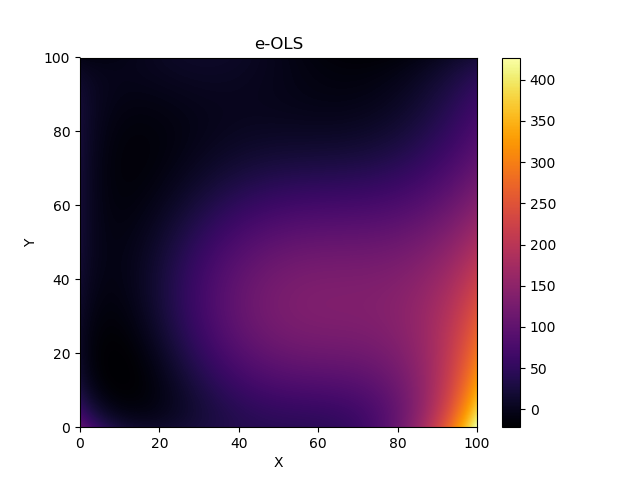
\includegraphics[scale=.7]{e-OLS}
\\Ridge:
\\ 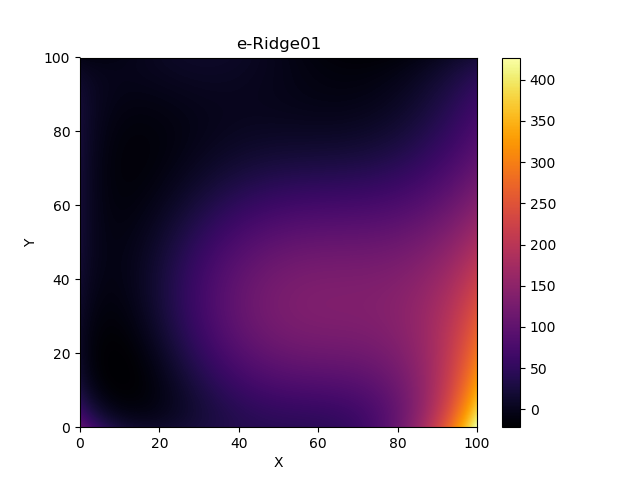
\includegraphics[scale=.7]{e-Ridge01}
\\Lasso:
\\ 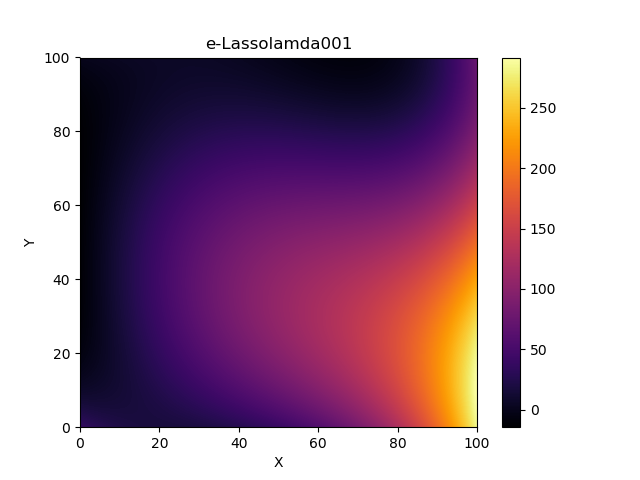
\includegraphics[scale=.7]{e-Lassolamda001}
\end{document}
